\documentclass{standalone}
\usepackage[dvipsnames, svgnames, x11names]{xcolor}
\usepackage{standalone}
\usepackage{tikz}
\usepackage{graphicx}
\usepackage{float}
\usepackage{listings}
\usepackage{caption}
\usepackage{fancyhdr}
\usetikzlibrary{decorations.pathreplacing,calligraphy}
\begin{document}
% \begin{framed}
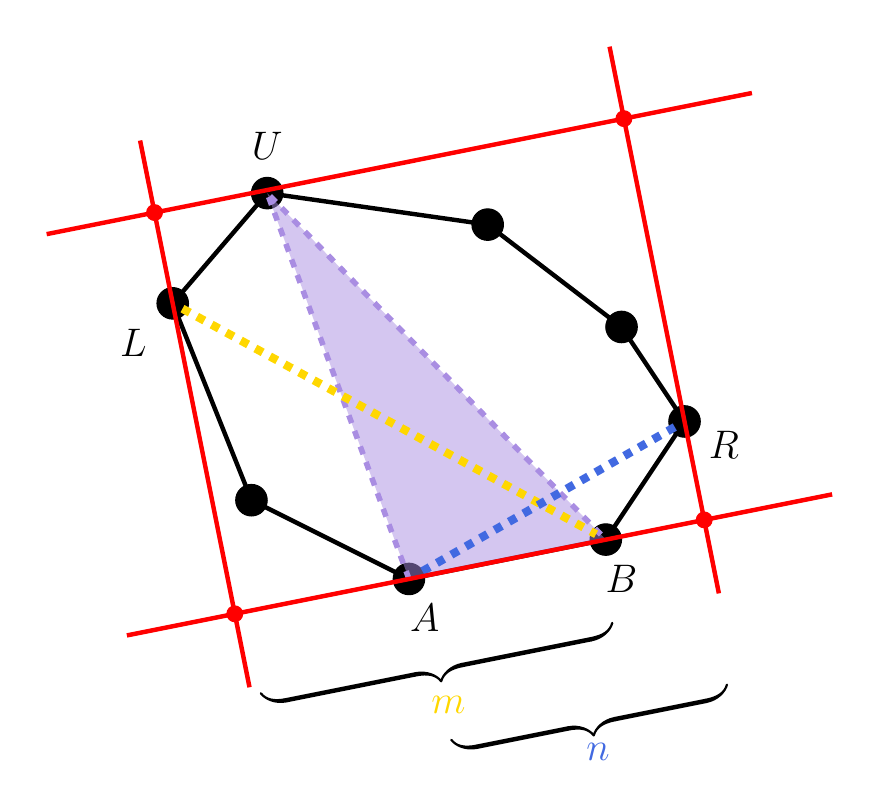
\begin{tikzpicture}
\node (A) at (4, 2.5) {};
\node (B) at (6.5, 3) {};
\node (R) at (7.5, 4.5) {};
\node (L) at (1, 6) {};
\node (C) at (6.7, 5.7) {};
\node (D) at (5, 7) {};
\node (U) at (2.2, 7.4) {};
\node (F) at (2, 3.5) {};

\node at (4.2,2) [font=\fontsize{14}{0}\selectfont] {$A$};
\node at (6.7, 2.5) [font=\fontsize{14}{0}\selectfont] {$B$};
\node at (8, 4.2) [font=\fontsize{14}{0}\selectfont] {$R$};
\node at (0.5, 5.5) [font=\fontsize{14}{0}\selectfont] {$L$};
\node at (2.2, 8) [font=\fontsize{14}{0}\selectfont] {$U$};

\filldraw (A) circle (.2) (B) circle (.2) (C) circle (.2) (D) circle (.2) (U) circle (.2) (F) circle (.2) (L) circle (.2) (R) circle (.2);

\draw[ultra thick] (A)--(B)--(R)--(C)--(D)--(U)--(L)--(F)--(A);

\node (P) at (0.561, 8.192) {};
\node (S) at (2.000, 1.000) {};
\node (Q) at (6.523, 9.384) {};
\node (T) at (7.961, 2.192) {};
\node (N) at (-0.725,6.854) {};
\node (O) at (8.480, 8.696) {};
\node (K) at (0.294, 1.758) {};
\node (M) at (9.499, 3.599) {};

\node (G) at (1.788, 2.057) {};
\node (H) at (7.750, 3.250) {};
\node (J) at (0.769, 7.153) {};
\node (I) at (6.730, 8.346) {};

\filldraw[color = red] (G) circle (.1) (H) circle (.1) (J) circle (.1) (I) circle (.1);

\filldraw[MediumPurple!80, fill opacity=0.5, dashed, line width=2, draw=MediumPurple!80] (A.center)--(U.center)--(B.center);

\draw[dashed, line width=3, draw=Gold1] (L)--(B);
\draw[dashed, line width=3, draw=RoyalBlue] (R)--(A);

\draw[decorate, decoration={mirror, calligraphic brace,amplitude=3mm, raise=30pt},ultra thick] (G)--(B);
\node at (4.5,0.9) [Gold1, font=\fontsize{14}{0}\selectfont] {$m$};
\draw[decorate, decoration={mirror, calligraphic brace,amplitude=3mm, raise=60pt},ultra thick] (A)--(H);
\node at (6.4,0.3) [RoyalBlue, font=\fontsize{14}{0}\selectfont] {$n$};
\draw[red, ultra thick] (P)--(S) (Q)--(T) (N)--(O) (K)--(M);


\end{tikzpicture}
% \end{framed}

\end{document}
